\section{INTRODUCTION}
\label{chap:introduction}

\section{Objectives of the museum visit}
\label{sec:objectives}

\begin{figure}[H]
  \centering
  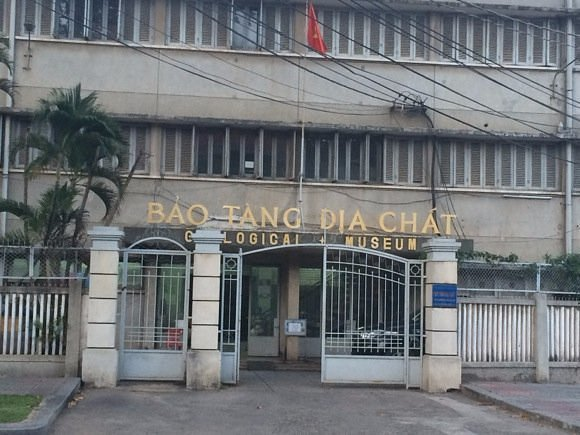
\includegraphics[width=0.8\textwidth]{graphics/figure_01.jpg}
  \caption{Ho Chi Minh City Geological Museum}
  \label{fig:museum}
\end{figure}

The visit to the Ho Chi Minh City Geological Museum provided us with a valuable chance to connect the theories we learned in class with real-world examples. While books and lectures give us the foundation of geological knowledge, nothing compares to directly observing the specimens that reflect millions, even billions, of years of Earth's history. At the museum, we could see how rocks, ores, minerals, and gemstones are preserved and displayed, each telling a story about the planet's formation and transformation over time.

This experience not only strengthened our understanding of the processes that shape the Earth but also gave us a clearer view of Vietnam's own geological heritage. By exploring these collections, we were able to develop a deeper appreciation of geology as both a science and a record of natural history. More importantly, the museum visit allowed us to practice critical observation, linking theory with practice, and to better prepare for future studies and projects related to Earth sciences.

\section{General history about Ho Chi Minh City Geological Museum}
\label{sec:history}

The Geological Museum has a long history closely tied to the development of geological research in Vietnam since the colonial period. In 1898, the French colonial government established the Indochina Geological Service (Service Géologique de l'Indochine) and initiated the construction of a museum dedicated to geological research and education. By 1914, the museum's first building was completed in Hanoi. After the Geneva Agreement in 1954, part of the collection was moved to Saigon, where it was initially displayed in a temporary villa before being relocated to its current building in 1973. Following national reunification, the museum was managed by the Southern Geological Mapping Federation and continued to expand within the national geological system.

In 2001, it became one of the first museums in Vietnam to be recognized by the International Council of Museums (ICOM). In 2003, the Geological Museum system was restructured under the Department of Geology and Minerals, and in 2008, the Ho Chi Minh City branch was officially integrated as the southern division. Today, the Geological Museum stands as Vietnam's national geological museum, operating under the Department of Geology and Minerals of the Ministry of Natural Resources and Environment.